\chapter{費米子質量：手徵性、湯川耦合與馬約拉納中微子}

\lectureoverview{我們先在玩具\(U(1)\)理論中重新推導規範玻色子的希格斯機制，再對費米子提出相應的問題。狄拉克質量會混合左、右手徵場，但弱相互作用賦予兩者不同的荷，因此禁止裸質量。與希格斯場的湯川耦合符合對稱性；希格斯場取得真空值後，同一個相互作用便成為費米子質量，以及可測量的希格斯--費米子耦合。最後一部分將沿著這個脈絡，探討中微子質量、可能存在的未受保護重粒子、宇宙射線運動學、相對論中的慣性，以及重力。}

開場回顧的目的不只是重述上一講的內容。我們需要從中提取一個可延伸至費米子的觀念：質量是零動量激發態所具有的非零能量。對場而言，零動量意味著無限波長，也就是處處相同的位移。只有導數項的理論無法感知均勻位移；不含導數的項則可以。

\section{規範玻色子的機制：快速回顧}

\subsection{導數能量與無質量向量場}

模型中的規範場是\(A_\mu\)，其場強為
\begin{equation}
  F_{\mu\nu}
  =\partial_\mu A_\nu-\partial_\nu A_\mu .
  \label{eq:l09-field-strength}
\end{equation}
黑板上以示意方式將規範場的動能項寫成\(F^2\)。採用標準歸一化後，它的形式為
\begin{equation}
  \mathcal L_{\mathrm{gauge}}
  =-\frac14 F_{\mu\nu}F^{\mu\nu}.
  \label{eq:l09-gauge-kinetic}
\end{equation}

\begin{figure}[htbp]
\centering
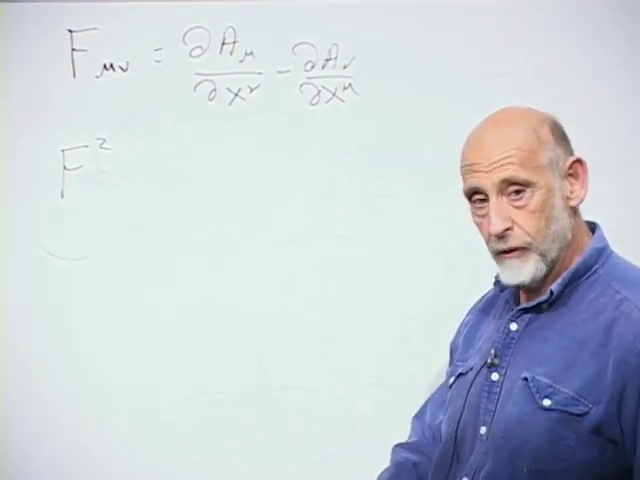
\includegraphics[width=0.72\textwidth]{lecture_09_figure_02.png}
\caption{場強的定義，以及黑板上以\(F^2\)表示規範場導數能量的簡寫。}
\lectureframe{00:02:39}
\label{fig:l09-field-strength-board}
\end{figure}

在\eqref{eq:l09-gauge-kinetic}中，每一個\(A_\mu\)都經過微分。因此，
\begin{equation}
  A_\mu(x)\longmapsto A_\mu(x)+c_\mu,
  \qquad \partial_\nu c_\mu=0,
\end{equation}
不會改變\(F_{\mu\nu}\)。所以，均勻的向量勢不會產生場強能量。用本講的說法，零動量模沒有能隙，規範玻色子因此是無質量的。

這個\(U(1)\)場是刻意簡化的替代模型。實際要討論的是\(W^\pm\)和\(Z\)，而非電磁光子。未破缺的電磁對稱性使光子保持無質量；電弱對稱性的破缺則使弱規範玻色子取得質量。

\subsection{凍結希格斯場的徑向自由度}

引入一個帶電複純量場，並將它寫成極座標形式：
\begin{equation}
  \phi(x)=\rho(x)e^{i\alpha(x)}.
\end{equation}
它的墨西哥帽勢在半徑非零的圓周上取極小值。將這個半徑記為\(f\)；徑向方向的變化相對而言代價較高。第一步先凍結徑向自由度，只保留相位：
\begin{equation}
  \phi(x)\simeq f e^{i\alpha(x)}.
  \label{eq:l09-frozen-higgs}
\end{equation}

\begin{figure}[htbp]
\centering
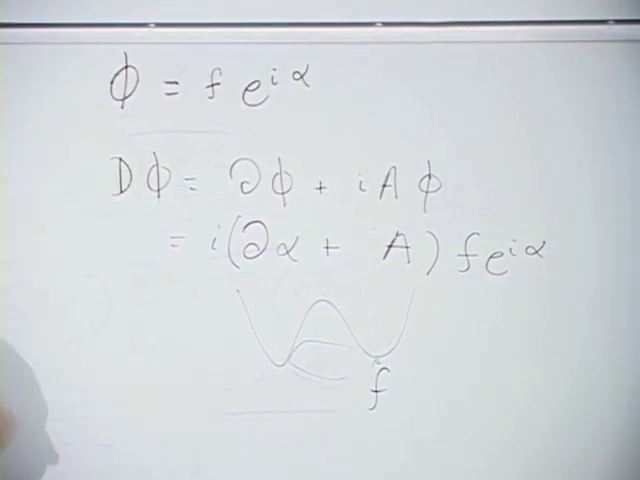
\includegraphics[width=0.72\textwidth]{lecture_09_figure_03.png}
\caption{凍結的希格斯場徑向自由度、其協變導數，以及回顧時使用的簡化破缺勢示意圖。}
\lectureframe{00:06:42}
\label{fig:l09-frozen-board}
\end{figure}

採用以下約定：
\begin{equation}
\begin{aligned}
  D_\mu&=\partial_\mu+igA_\mu,
  \\
  \phi&\longmapsto e^{i\theta}\phi,
  \\
  A_\mu&\longmapsto A_\mu-\frac1g\partial_\mu\theta .
\end{aligned}
  \label{eq:l09-gauge-convention}
\end{equation}
本講省略了\(g\)；將它明確寫出，量綱和最後得到的質量便一目了然。協變導數作用在凍結的場上，得到
\begin{align}
  D_\mu\phi
  &=(\partial_\mu+igA_\mu)f e^{i\alpha}
  \notag\\
  &=i\bigl(\partial_\mu\alpha+gA_\mu\bigr)
    f e^{i\alpha}.
  \label{eq:l09-covariant-frozen}
\end{align}
乘上複共軛後，相位會消去，而\(i\)與\(-i\)相乘也會得到\(+1\)：
\begin{equation}
  |D_\mu\phi|^2
  =f^2
   \bigl(\partial_\mu\alpha+gA_\mu\bigr)
   \bigl(\partial^\mu\alpha+gA^\mu\bigr).
  \label{eq:l09-frozen-square}
\end{equation}

\begin{classroomqa}
\audiencequestion{協變導數的平方是否應該帶負號？畢竟微分後會出現\(i\)因子。
\lecturetimestamp{00:07:39}}
\lecturerresponse{不需要。動能項是協變導數與其複共軛的乘積。一個因子帶來\(i\)，另一個帶來\(-i\)，而\(i(-i)=1\)。\(D_\mu\)的符號約定可以一致地反轉，但相應能量表達式中的模平方仍為正。}
\end{classroomqa}

\eqref{eq:l09-frozen-square}中的組合本身就是經過位移的規範場。選擇\(\theta=-\alpha\)，使純量場的相位消去，並定義
\begin{equation}
  A'_\mu=A_\mu+\frac1g\partial_\mu\alpha .
  \label{eq:l09-unitary-gauge-field}
\end{equation}
於是
\begin{equation}
  |D_\mu\phi|^2=g^2f^2 A'_\mu A'^\mu .
  \label{eq:l09-vector-mass-term}
\end{equation}
新項不含\(A'_\mu\)的導數。均勻場現在具有能量，因此零動量向量模出現能隙。

\begin{figure}[htbp]
\centering
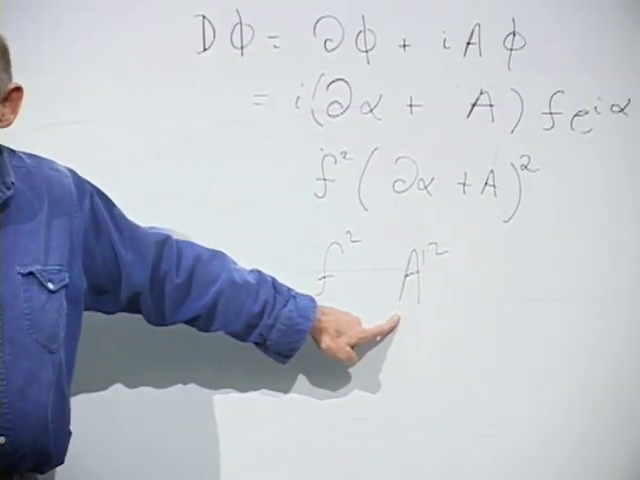
\includegraphics[width=0.72\textwidth]{lecture_09_figure_04.png}
\caption{黑板上單獨列出\(f^2A^2\)項；相位吸收後，這一項標示出規範玻色子質量的產生。}
\lectureframe{00:10:31}
\label{fig:l09-vector-mass-board}
\end{figure}

採用正則純量場歸一化時，可寫成
\(\phi=(f+h)e^{i\pi/f}/\sqrt2\)。將得到的向量場項與
\(\tfrac12m_A^2A_\mu A^\mu\)相比，可得
\begin{equation}
  m_A=gf
  \label{eq:l09-abelian-vector-mass}
\end{equation}
這就是此阿貝爾模型中的結果。本講略去歸一化因子，並以向量場質量由\(f\)決定來概括。

相位模並非無故消失。在規範化之前，它是無質量的戈德斯通玻色子；規範化之後，它提供了有質量向量粒子所需的縱向偏振自由度。我們暫時凍結的徑向漲落，則保留為物理希格斯激發。

\subsection{為什麼不含導數的項代表質量}

\begin{classroomqa}
\audiencequestion{為什麼\(A'^2\)項代表質量，而不只是另一種相互作用？\lecturetimestamp{00:13:10}}
\lecturerresponse{質量就是靜止能量。對場而言，靜止粒子是零動量、無限波長模態的量子。導數項不會讓靜止的均勻位移具有能量，但\(m_A^2A'^2\)會。這個零動量時仍存在的非零能量，就是靜止能量的能隙。}
\end{classroomqa}

本講透過三個力學類比來說明這一點。

\begin{itemize}
  \item 在晶體中，緩慢變化的位移會產生彈性能，因為相鄰原子的位移不同。若所有原子一起剛性平移，則不會產生內能。因此，聲學聲子沒有能隙。
  \item 在理想的旋轉對稱磁體中，空間變化的自旋方向會產生交換能；若所有自旋一起旋轉，則不會。相應的長波長自旋波沒有能隙。
  \item 在電漿中，電子流體相對於正電荷背景發生位移會造成電荷分離，並產生恢復電場；即使相對位移是均勻的，情況也是如此。因此，等離激元在零波數時仍具有非零頻率。
\end{itemize}

希格斯機制下的規範場表現得像第三個例子：破缺後的介質會抵抗原本不需付出能量的均勻位移。

\begin{classroomqa}
\audiencequestion{引入規範場之前，相位\(\alpha\)不是已經會振動了嗎？\lecturetimestamp{00:18:24}}
\lecturerresponse{會。它的能量正比於\(f^2(\partial_\mu\alpha)^2\)。相位若隨位置變化，便具有梯度能量，也能傳播；但均勻改變相位不需付出能量。這正是無質量的戈德斯通模態。}
\end{classroomqa}

\begin{classroomqa}
\audiencequestion{導數中也包含時間導數。若真的移動整個晶格，或改變整個場，難道不會帶有動能嗎？\lecturetimestamp{00:22:18}}
\lecturerresponse{會。這裡比較的是靜態構型，或以任意緩慢的方式準備出的構型。晶格若以非零速度平移，就具有動能。判斷質量時要問的是：構型處於靜止且空間均勻時，是否仍具有能量。}
\end{classroomqa}

\section{實驗線索：弱相互作用區分左右}

接著轉向電子、{\proseunicodefont μ}子和夸克。它們的質量也來自希格斯場，但機制看起來不同，因為費米子質量不是向量場的二次項，而是兩個手徵場之間的耦合。

\subsection{{\proseunicodefont β} 衰變中的宇稱破壞}

先從弱相互作用會破壞宇稱這項實驗事實談起。量子電動力學和量子色動力學對某個過程及其鏡像過程一視同仁；弱相互作用則不然。在中子 {\proseunicodefont β} 衰變中，
\begin{equation}
  n\longrightarrow p+e^-+\bar\nu_e,
  \label{eq:l09-beta-decay}
\end{equation}
帶電流相互作用所選出的高能電子具有左手螺旋度：它們的自旋方向與動量方向相反。相應的反中微子則具有相反的螺旋度。

對超相對論粒子，螺旋度定義為
\begin{equation}
  h=\frac{\bm S\cdot\bm p}{|\bm S|\,|\bm p|}.
\end{equation}
自旋平行於動量時，螺旋度為\(h=+1\)；自旋反平行於動量時，則為\(h=-1\)。
弱相互作用會耦合到左手徵電子場與左手徵中微子場，但不會以相同方式耦合到右手徵電子場。\editorialnote{本講一開始用螺旋度來談左右手性，因為在高能下這種說法直觀易懂。但規範荷實際作用於手徵性，也就是由\(P_L=(1-\gamma^5)/2\)和\(P_R=(1+\gamma^5)/2\)選定的洛侖茲表示標籤。對無質量粒子而言，粒子的手徵性與螺旋度一致；對有質量粒子而言，兩者則不相同。}

為了不必處理完整的\(SU(2)_L\times U(1)_Y\)記號，就能看出這個障礙，可以設想一個虛構的\(U(1)\)世界，其中只有\(\psi_L\)帶有相關的荷：
\begin{equation}
  \psi_L\longmapsto e^{i\theta}\psi_L,
  \qquad
  \psi_R\longmapsto\psi_R .
  \label{eq:l09-chiral-toy-charge}
\end{equation}
這不是電磁學；真實的左、右手徵電子帶有相同的電荷。這只是弱相互作用的簡化圖像：兩種手徵性屬於不同的電弱表示。

\begin{classroomqa}
\audiencequestion{夸克也有相同的左--右不對稱性嗎？\lecturetimestamp{00:31:50}}
\lecturerresponse{有，但須考慮適當的弱多重態和超荷。左手徵的上型與下型夸克組成弱二重態，右手徵場則是弱單態。因此，它們的希格斯耦合同樣面臨與電子相同的結構性問題。}
\end{classroomqa}

\section{狄拉克質量會混合左--右}

\subsection{從四分量方程到兩個韋爾方程}

狄拉克波函數有四個分量。粗略而言，其中兩個描述自旋，另外兩個區分正能量解與負能量解；後者重新詮釋為反粒子的自由度。寫成哈密頓形式：
\begin{equation}
  i\frac{\partial\Psi}{\partial t}
  =\left(-i\bm\alpha\cdot\bm\nabla+m\beta\right)\Psi .
  \label{eq:l09-dirac-hamiltonian}
\end{equation}
矩陣\(\alpha_i\)和\(\beta\)表現了能量、動量與質量之間的相對論關係。

\begin{figure}[htbp]
\centering
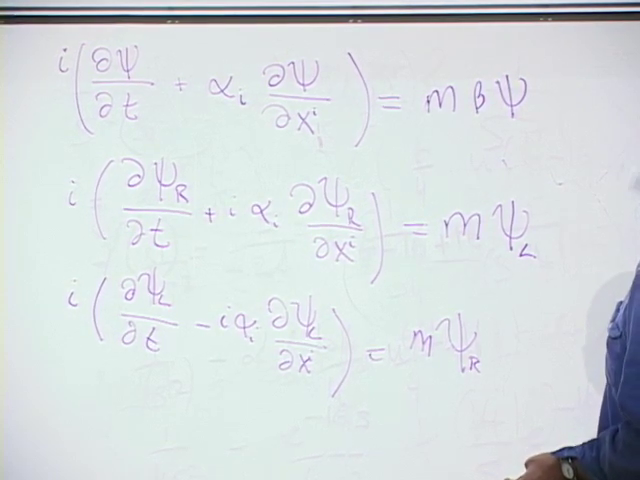
\includegraphics[width=0.74\textwidth]{lecture_09_figure_05.png}
\caption{黑板上先寫出狄拉克方程，再將它拆解為彼此耦合的左、右手徵方程。}
\lectureframe{00:40:30}
\label{fig:l09-dirac-board}
\end{figure}

手徵基底明確呈現了\(m\)的作用。令
\(\sigma^\mu=(1,\bm\sigma)\)和
\(\bar\sigma^\mu=(1,-\bm\sigma)\)，則
\begin{align}
  i\bar\sigma^\mu\partial_\mu\psi_L&=m\psi_R,
  \label{eq:l09-weyl-left}\\
  i\sigma^\mu\partial_\mu\psi_R&=m\psi_L.
  \label{eq:l09-weyl-right}
\end{align}
當\(m=0\)時，兩個方程彼此獨立：左手徵場和右手徵場可以各自傳播，互不耦合。當\(m\neq0\)時，每個場都成為另一個場的源。這就是狄拉克質量混合左右手徵場的確切含義。

Susskind將此描述為費米子在左右手徵之間振盪。這種說法點出了耦合，但不應將它延伸成點粒子來回翻轉的字面圖像。精確的說法是，場方程彼此耦合：
\eqref{eq:l09-weyl-left}--\eqref{eq:l09-weyl-right}。

\begin{classroomqa}
\audiencequestion{黑板上兩個方程中的\(i\)因子和符號是否一致？\lecturetimestamp{00:41:10}}
\lecturerresponse{黑板上的寫法並非逐行一致；快速推導時，有一個\(i\)被不一致地提出方程之外。可靠的內容是耦合的形式。方程\eqref{eq:l09-weyl-left}和
\eqref{eq:l09-weyl-right}給出一套標準且一致的約定。}
\end{classroomqa}

\subsection{為什麼弱對稱性禁止裸質量}

相應的狄拉克質量項在拉格朗日量中寫為
\begin{equation}
  \mathcal L_m
  =-m\bar\psi\psi
  =-m\left(\bar\psi_L\psi_R+\bar\psi_R\psi_L\right).
  \label{eq:l09-bare-dirac-mass}
\end{equation}
在玩具模型的變換\eqref{eq:l09-chiral-toy-charge}下，
\begin{equation}
  \bar\psi_L\psi_R\longmapsto
  e^{-i\theta}\bar\psi_L\psi_R,
  \qquad
  \bar\psi_R\psi_L\longmapsto
  e^{i\theta}\bar\psi_R\psi_L.
\end{equation}
兩項都不是不變量。因此，在對稱性破缺之前，直接混合左--右手徵場的係數\(m\)會受到禁止。

單靠電磁作用不會造成這個問題，因為\(\psi_L\)和\(\psi_R\)具有相同的電荷。這個障礙源自兩者不同的弱量子數。

\subsection{揭示手徵性微妙之處的螺旋度問題}

接著，課堂從幾個角度檢驗直觀的左右手性圖像。這些問題並非枝節；它們正好揭示螺旋度在哪些情況下有用，又在哪些情況下必須改以手徵性來描述。

\begin{classroomqa}
\audiencequestion{如果弱相互作用以相同的機率產生兩種螺旋度的電子，世界會是什麼樣子？\lecturetimestamp{00:42:12}}
\lecturerresponse{該過程中的宇稱不對稱性會立即消失。但真實的電弱理論具有手徵性：只有左手徵二重態帶有帶電流弱相互作用。至於自然界為何採取這種結構，本講將延後再作更完整的說明。}
\end{classroomqa}

\begin{classroomqa}
\audiencequestion{假設電子的自旋沿垂直方向準備，接著電子沿水平方向加速。它是左手性還是右手性？\lecturetimestamp{00:42:44}}
\lecturerresponse{自旋若垂直於動量方向，該自旋態就是兩種螺旋度的疊加。只有當自旋平行或反平行於動量時，螺旋度才有確定值。不過，對場而言，弱手徵投影算符仍有明確定義。}
\end{classroomqa}

有質量粒子可以減速至靜止，再沿相反方向加速，而自旋方向保持不變。此時它的螺旋度會改變符號。無質量粒子無法被洛侖茲推進追上或帶至靜止，因此其螺旋度在固有推進下保持不變。這是本講所說「只有一種物理螺旋度的粒子種類必須無質量」的理由。更精確的場論說法是，洛侖茲不變的狄拉克質量需要兩種手徵性。

\begin{classroomqa}
\audiencequestion{圓偏振光子可以從鏡面反射，改變傳播方向，卻從未靜止。這是否與螺旋度論證矛盾？\lecturetimestamp{00:45:28}}
\lecturerresponse{不矛盾。鏡子是外部系統，可以交換角動量並反轉傳播方向。反射過程並不是透過洛侖茲推進追上光子。某個通道是否存在，也取決於允許的偏振態和材料的邊界條件。}
\end{classroomqa}

\begin{classroomqa}
\audiencequestion{一般的電子束具有一種手性，還是兩種都有？\lecturetimestamp{00:46:10}}
\lecturerresponse{一般而言，兩種都有。有質量電子態包含兩種手徵分量，而未偏振的電子束包含兩種螺旋度。專用的電子源則可以產生螺旋度不對稱性很大的偏振束。}
\end{classroomqa}

\begin{classroomqa}
\audiencequestion{束流能否在不受自旋影響的情況下聚焦？還是磁場會將兩種偏振分開？\lecturetimestamp{00:46:29}}
\lecturerresponse{一般的位置聚焦大致上可以不受自旋影響，但磁矩會與磁場梯度耦合。因此，自旋選擇性電子源、類似斯特恩--格拉赫實驗的磁場梯度，以及加速器中的自旋動力學，都可以用來製備或分離不同偏振態。}
\end{classroomqa}

\begin{classroomqa}
\audiencequestion{弱相互作用對左右的差異只是偶然嗎？\lecturetimestamp{00:48:13}}
\lecturerresponse{就本課程而言，這是納入標準模型的實驗事實。其規律性如此強，不像隨意的偶然；但標準模型本身並未從更深層的原理推導出完整的手徵荷排列。}
\end{classroomqa}

\section{湯川耦合的建構}

\subsection{讓希格斯場帶有缺少的荷}

對稱性禁止直接加入數值質量，卻允許與某個場相互作用，由該場提供缺少的變換相位。引入一個複純量場，使其滿足
\begin{equation}
  \phi\longmapsto e^{i\theta}\phi,
  \qquad
  \phi^\dagger\longmapsto e^{-i\theta}\phi^\dagger.
  \label{eq:l09-scalar-charge}
\end{equation}
則
\begin{equation}
  \mathcal L_Y
  =-y\,\bar\psi_L\phi\psi_R
   -y^*\,\bar\psi_R\phi^\dagger\psi_L
  \label{eq:l09-yukawa-lagrangian}
\end{equation}
便具有規範不變性。在第一項中，
\(\bar\psi_L\)帶來\(e^{-i\theta}\)，而\(\phi\)帶來\(e^{i\theta}\)；兩個相位彼此抵消。第二項是其厄米共軛。

等價地，手徵方程中會出現依賴場的混合項：
\begin{align}
  i\bar\sigma^\mu D_\mu\psi_L
    &=y\phi\psi_R,
  \label{eq:l09-yukawa-eom-left}\\
  i\sigma^\mu\partial_\mu\psi_R
    &=y^*\phi^\dagger\psi_L.
  \label{eq:l09-yukawa-eom-right}
\end{align}

\begin{figure}[htbp]
\centering
\includegraphics[width=0.76\textwidth]{lecture_09_figure_06.png}
\caption{方程右側的裸質量已由帶電純量場取代。黑板上的具體符號僅為示意；不變的結構見\eqref{eq:l09-yukawa-lagrangian}。}
\lectureframe{00:51:30}
\label{fig:l09-yukawa-board}
\end{figure}

對稱性破缺之前，這是一種相互作用，而非質量。右手徵費米子只有在發射或吸收用來平衡荷的純量量子時，才能轉變為左手徵費米子。係數\(y\)是湯川耦合，不是規範荷\(g\)。

\begin{classroomqa}
\audiencequestion{直接將\(\phi\)和\(\phi^\dagger\)放在兩個方程右側，這樣合理嗎？
\lecturetimestamp{00:51:55}}
\lecturerresponse{合理，正是因為它們的變換相位補上了不匹配之處。關鍵不在方程表面上的形式，而在於相互作用\(\bar\psi_L\phi\psi_R+\mathrm{h.c.}\)是否具有規範不變性。}
\end{classroomqa}

\subsection{真空將相互作用轉化為質量}

現在將\(\phi\)視為希格斯場，並讓它穩定在非零的真空幅值。在本講採用的簡化歸一化下，
\begin{equation}
  \phi\simeq f,
\end{equation}
因此\eqref{eq:l09-yukawa-lagrangian}包含
\begin{equation}
  \mathcal L_Y
  \supset
  -yf\,\bar\psi_L\psi_R
  -y^*f\,\bar\psi_R\psi_L .
\end{equation}
在適當的情況下，經過不影響物理的相位重新定義後，費米子質量為
\begin{equation}
  m_f=yf.
  \label{eq:l09-lecture-fermion-mass}
\end{equation}
這是向量場結果\(m_A=gf\)在費米子上的對應。為弱規範玻色子提供縱向偏振自由度的同一個希格斯真空，也提供了連結左、右手徵費米子所需的弱量子數。

採用標準模型的正則歸一化慣例時，
\begin{equation}
  H(x)=\frac1{\sqrt2}
  \begin{pmatrix}
    0\\ v+h(x)
  \end{pmatrix},
  \qquad v\simeq246\ \mathrm{GeV},
  \label{eq:l09-sm-higgs-vacuum}
\end{equation}
因此
\begin{equation}
  m_f=\frac{y_fv}{\sqrt2}.
  \label{eq:l09-sm-fermion-mass}
\end{equation}
本講採用的\(f\)與慣用的\(v/\sqrt2\)僅在歸一化選擇上有所不同。

\begin{classroomqa}
\audiencequestion{如果只有乘積\(yf\)才是費米子質量，如何分別求出耦合\(y\)與真空尺度\(f\)？
\lecturetimestamp{00:55:36}}
\lecturerresponse{已知規範耦合後，弱規範玻色子的質量可以決定真空尺度；再由費米子的測得質量決定其湯川耦合。在完整理論中，
\(m_W=gv/2\)、\(m_Z=v\sqrt{g^2+g'^2}/2\)和\(y_f=\sqrt2m_f/v\)。}
\end{classroomqa}

\begin{classroomqa}
\audiencequestion{弱玻色子的質量大約是\(900\ \mathrm{GeV}\)嗎？\lecturetimestamp{00:57:43}}
\lecturerresponse{不是；講座隨即更正口誤，指出大約是\(90\ \mathrm{GeV}\)。更精確地說，
\(m_W\simeq80\ \mathrm{GeV}\)和\(m_Z\simeq91\ \mathrm{GeV}\)，而真空的基本尺度為\(v\simeq246\ \mathrm{GeV}\)。}
\end{classroomqa}

\subsection{一個真空尺度，多種湯川耦合}

每一種帶電費米子都有各自的湯川耦合：
\begin{equation}
  m_i=y_i f
  \qquad\text{(lecture normalization)}.
  \label{eq:l09-mass-family}
\end{equation}

\begin{figure}[htbp]
\centering
\includegraphics[width=0.76\textwidth]{lecture_09_figure_08.png}
\caption{黑板以\(m_i=g_i f\)概括不同粒子的差異；其中的\(g_i\)就是此處所稱的湯川耦合\(y_i\)。}
\lectureframe{01:16:30}
\label{fig:l09-mass-family-board}
\end{figure}

本講估算電子的湯川耦合為
\begin{equation}
  y_e\sim\frac{0.5\ \mathrm{MeV}}{10^2\ \mathrm{GeV}}
  \sim10^{-5}.
\end{equation}
使用正則歸一化的數值\(v=246\ \mathrm{GeV}\)後，可得更精確的結果：
\(y_e\simeq2.9\times10^{-6}\)。頂夸克則位於另一個極端：
\begin{equation}
  y_t=\frac{\sqrt2m_t}{v}\simeq1.
\end{equation}
因此，希格斯機制解釋了規範不變的質量如何存在，卻沒有解釋各個\(y_i\)之間為何有如此巨大的階層差異。觀測到的費米子質量只是把這種差異呈現為測量數值。

\begin{classroomqa}
\audiencequestion{頂夸克的湯川耦合真的約為一嗎？\lecturetimestamp{00:59:09}}
\lecturerresponse{是的。頂夸克的質量與電弱尺度相當，因此其耦合不像電子的耦合那樣微小。在現代的歸一化慣例下，\(y_t\)接近一。}
\end{classroomqa}

\subsection{恢復物理的希格斯場漲落}

將純量場凍結在真空值，會把徑向激發隱藏起來。現在以示意方式將它恢復：
\begin{equation}
  \phi(x)\simeq f+h(x).
\end{equation}
湯川因子便成為
\begin{equation}
  y\phi\simeq yf+yh=m_f+yh.
  \label{eq:l09-mass-plus-higgs}
\end{equation}

\begin{figure}[htbp]
\centering
\includegraphics[width=0.76\textwidth]{lecture_09_figure_07.png}
\caption{黑板上的湯川項恢復了希格斯場漲落：常數部分產生費米子質量，漲落部分則讓希格斯玻色子得以發射或吸收。}
\lectureframe{01:01:15}
\label{fig:l09-higgs-fluctuation-board}
\end{figure}

\eqref{eq:l09-mass-plus-higgs}中的第一項是質量項。第二項則是希格斯玻色子與費米子耦合的頂點。採用標準模型的慣用記法時，
\begin{equation}
  \mathcal L_Y
  \supset
  -m_f\bar\psi\psi
  -\frac{m_f}{v}h\bar\psi\psi.
  \label{eq:l09-higgs-fermion-vertex}
\end{equation}
此耦合正比於費米子質量。因此，考量運動學、色因子、相空間及其他競爭衰變道後，希格斯與較重費米子的耦合會較強。

\begin{classroomqa}
\audiencequestion{耦合常數本身就是機率嗎？\lecturetimestamp{01:03:35}}
\lecturerresponse{耦合常數會出現在量子振幅中。簡單的反應率通常正比於振幅的模平方，因此也會正比於耦合常數的平方；但相空間、自旋求和、干涉、圈圖及多個頂點也都會產生影響。不能直接把耦合常數等同於機率。}
\end{classroomqa}

\begin{classroomqa}
\audiencequestion{這套論證是否假設只有一個希格斯場？\lecturetimestamp{01:03:59}}
\lecturerresponse{這裡描述的是最小標準模型，其中包含一個複希格斯二重態。它的四個實分量中，有三個被\(W^\pm\)和\(Z\)吸收，剩下一個物理的中性純量。延伸模型可以包含更多二重態或其他純量多重態。超對稱模型通常需要兩個希格斯二重態，因此會有數個物理希格斯態。}
\end{classroomqa}

現在可以將當時的預期與實驗結果相比較。
\editorialnote{本講錄製於希格斯玻色子發現之前。ATLAS 和 CMS 在2012年宣布發現類希格斯粒子；如今測得其質量接近\(125\ \mathrm{GeV}\)。觀測到的耦合大致符合標準模型中耦合與質量成正比的模式。所謂希格斯優先衰變至最重粒子的說法，始終受運動學條件限制：在殼的\(t\bar t\)對，其質量對\(125\ \mathrm{GeV}\)希格斯玻色子而言過重，無法產生。}

\section{反粒子、束流與手徵性的意義}

轉向中微子之前，課堂先回到幾個關於反粒子與加速器束流的實際問題。

\begin{classroomqa}
\audiencequestion{左手徵電子的反粒子具有什麼手徵性？\lecturetimestamp{01:06:05}}
\lecturerresponse{在超相對論極限下，左手徵電子場會湮滅左手螺旋度電子，並產生右手螺旋度正電子。這正是必須仔細說明粒子與反粒子、手徵性與螺旋度之間差異的例子之一。}
\end{classroomqa}

\begin{classroomqa}
\audiencequestion{電子和正電子能否碰撞產生\(Z\)玻色子？\lecturetimestamp{01:07:13}}
\lecturerresponse{可以，前提是它們的質心能量符合該反應道的條件。電子--正電子對撞機曾以極高精度研究\(Z\)共振。整個過程中的電荷及其他量子數都守恆。}
\end{classroomqa}

\begin{classroomqa}
\audiencequestion{正電子是否都透過某種特殊的弱作用過程產生？\lecturetimestamp{01:07:37}}
\lecturerresponse{不是。成對產生是標準的電磁途徑之一。例如，高能電子可以放出虛光子，而該光子能在另一粒子的場中產生\(e^-e^+\)對。本講以費曼圖示意這個過程。}
\end{classroomqa}

\begin{classroomqa}
\audiencequestion{直線加速器能選擇電子的速度或能量嗎？\lecturetimestamp{01:09:24}}
\lecturerresponse{可以。加速場和定時控制可選出一段能量範圍。電子進入超相對論狀態後，速度已極為接近\(c\)；因此，增加加速器能量主要提高其動量和總能量，而不會明顯提高速度。}
\end{classroomqa}

\begin{classroomqa}
\audiencequestion{加速器能製備單一偏振態的束流嗎？\lecturetimestamp{01:09:47}}
\lecturerresponse{可以，但技術上相當困難。可先在低能量下使用自旋依賴的電子源，製備自旋偏極電子，再在控制自旋進動的同時加速。現代對撞機會測量所得束流的偏極度，而不會將其視為完全純的偏振態。}
\end{classroomqa}

\section{中微子質量與馬約拉納的可能性}

\subsection{為什麼中微子質量需要擴展標準模型}

最初的最小標準模型只包含左手徵中微子場，因此預測中微子無質量。中微子振盪顯示，至少有兩個中微子質量本徵值不同；這也表示中微子具有非零質量，儘管其質量與帶電費米子相比極小。

\begin{classroomqa}
\audiencequestion{中微子質量有多小？它們的右手分量在哪裡？\lecturetimestamp{01:10:38}}
\lecturerresponse{振盪實驗測得的是質量平方差，而非絕對質量。相應的質量尺度約為\(0.009\ \mathrm{eV}\)和\(0.05\ \mathrm{eV}\)。狄拉克描述會加入惰性的右手徵中微子；馬約拉納描述則將缺少的手徵性與電荷共軛的中微子場聯繫起來。}
\end{classroomqa}

若採用狄拉克中微子描述，就加入新的場\(\nu_R\)，並沿用湯川耦合的建構方式：
\begin{equation}
  \mathcal L_{\nu,\mathrm{Dirac}}
  =-y_\nu\bar L\,\widetilde H\,\nu_R+\mathrm{h.c.},
  \qquad
  m_\nu=\frac{y_\nu v}{\sqrt2}.
  \label{eq:l09-dirac-neutrino}
\end{equation}
所需的\(y_\nu\)極其微小。

還有另一種邏輯上的可能性，因為中微子不帶電荷。左手徵中微子可以與自身的電荷共軛態耦合，而後者具有相反的手徵性：
\begin{equation}
  \nu_L\longleftrightarrow(\nu_L)^c_R .
  \label{eq:l09-majorana-mixing}
\end{equation}
以這種方式構成的質量本徵態是馬約拉納費米子：除相位約定外，它就是自身的反粒子。類似的電子--正電子混合則不被允許，因為這會違反精確的電荷守恆。

\begin{classroomqa}
\audiencequestion{為什麼中微子允許粒子--反粒子混合，電子卻不允許？\lecturetimestamp{01:13:43}}
\lecturerresponse{電子和正電子帶有相反的電荷，因此，若以質量項將它們混合成同一個單粒子態，就會違反未破缺的電磁對稱性。中微子則不帶電。若沒有精確守恆的輕子數將中微子與其反粒子區分開來，馬約拉納質量便是允許的。}
\end{classroomqa}

這個名稱是為了紀念埃托雷·馬約拉納。這位年輕的義大利物理學家提出了這種實費米子表示法，並於1938失蹤。講座在此提及這個歷史謎團：他的下落始終未明。
\editorialnote{在電弱對稱性破缺之前，標準模型的活躍中微子並沒有可重整化且規範不變的裸馬約拉納質量項。在低能下，這種質量可以來自五維溫伯格算符\((LH)(LH)/\Lambda\)，也可以透過涉及重惰性中微子的蹺蹺板機制產生。中微子究竟是狄拉克粒子還是馬約拉納粒子，實驗上仍未有定論。}

\section{為什麼熟悉的粒子譜集中在電弱能標附近}

\subsection{共同能標及其重要限定}

\begin{classroomqa}
\audiencequestion{為什麼人們預期希格斯質量可在弱能標附近測得？\lecturetimestamp{01:14:48}}
\lecturerresponse{希格斯勢的曲率決定希格斯徑向模的質量，而同一個真空能標\(f\)則決定\(W\)和\(Z\)的質量。因此，若標量自耦合不極端，人們便預期希格斯質量與弱能標大致處於同一量級。觀測到的\(125\ \mathrm{GeV}\)確實落在這個範圍內。}
\end{classroomqa}

講座以一個醒目的總結指出，最小標準模型中的基本粒子質量，都可追溯至同一個破缺真空：
\begin{align}
  m_W&=\frac12gv,\\
  m_Z&=\frac12\sqrt{g^2+g'^2}\,v,\\
  m_f&=\frac1{\sqrt2}y_fv.
  \label{eq:l09-electroweak-mass-summary}
\end{align}
若\(v\)為零，而無因次耦合保持不變，弱規範玻色子和帶電基本費米子就都會是無質量的。

這個說法的適用範圍有限，不應任意擴大。光子和膠子仍然無質量，因為未破缺的規範對稱性保護著它們。質子和中子的大部分質量來自 QCD 束縛能，而不是夸克希格斯質量的總和。中微子質量則需要擴充最小模型。希格斯質量本身取決於標量勢，並非只是另一種湯川質量。

\subsection{質量不必等到對稱性破缺才產生的粒子}

假設某種新費米子的左手徵與右手徵分量具有相同的規範量子數，那麼
\(\bar\Psi_L\Psi_R+\mathrm{h.c.}\)本身就已是規範不變的。這種\emph{向量型}費米子可以具有與\(v\)無關的裸質量\(M\)：
\begin{equation}
  \mathcal L_{\mathrm{vectorlike}}
  =-M\bar\Psi\Psi.
  \label{eq:l09-vectorlike-mass}
\end{equation}
對於\(M\gg v\)，電弱對稱性並不會構成障礙。

這引出了講座對自然性的概括論證。受到規範對稱性或手徵對稱性保護的粒子，在希格斯真空破壞這種保護之前都保持無質量，因此其質量與相對較小的能標\(v\)相連。沒有這類保護的粒子則可能自然地重得多，因而不出現在觀測到的低能粒子譜中。我們所觀察到的粒子或許反映了一種選擇效應：能夠被探測到的粒子，正是那些質量必須等到電弱對稱性破缺才產生的粒子。

\begin{classroomqa}
\audiencequestion{具有獨立且大得多質量的粒子，在現實中就完全不起作用嗎？\lecturetimestamp{01:19:39}}
\lecturerresponse{它們難以產生，因此在一般的低能實驗室物理中作用不大，但仍可能影響高能歷程或宇宙學。講座以暗物質為例，指出較重的隱藏粒子譜或許會先在這個領域顯露。}
\end{classroomqa}

2010年的討論反映了當時流行的一種預期：暗物質粒子可能具有弱能標或稍高的質量。這仍是一類有用的模型，但不是已確立的事實。暗物質已透過引力效應被探測到，但其粒子身分及質量起源仍然未知。

\section{結語提問：宇宙射線、慣性、引力與手徵性}

\subsection{質量不等於高實驗室能量}

\begin{classroomqa}
\audiencequestion{宇宙射線的質量是多少？
\lecturetimestamp{01:20:57}}
\lecturerresponse{宇宙射線可能是質子、原子核、電子或光子；其不變質量就是該粒子或系統的不變質量。真正驚人的是它在實驗室參考系中的能量；能量最高的事件約可達\(10^{20}\)至\(10^{21}\ \mathrm{eV}\)。高能量不等於高不變質量。}
\end{classroomqa}

宇宙射線撞上近似靜止的靶粒子。若入射質子的實驗室能量為\(E\gg m_p\)，
\begin{equation}
  s=(p_1+p_2)^2
  \simeq2m_pE+2m_p^2,
  \qquad
  \sqrt{s}\simeq\sqrt{2m_pE}.
  \label{eq:l09-fixed-target-s}
\end{equation}
入射能量只有平方根的量級會轉化為質心能量。若兩束對撞粒子的能量相同，且各為\(E_{\rm beam}\)，
\begin{equation}
  \sqrt{s}\simeq2E_{\rm beam}.
  \label{eq:l09-collider-s}
\end{equation}
這就是對撞機將受控束流能量轉化為新粒子質量時，遠比固定靶實驗有效率的原因。

\begin{classroomqa}
\audiencequestion{為什麼 CERN 的對撞機會比單一粒子以高得多的能量撞擊靜止物質更有力？
\lecturetimestamp{01:21:50}}
\lecturerresponse{在固定靶碰撞中，動量守恆使末態的大部分實驗室能量仍以整體運動的形式向前傳遞。在對稱對撞機中，系統的總空間動量可以為零，因此束流能量可用作質心能量。能量最高的宇宙射線在\(\sqrt{s}\)方面仍可能超過 LHC，但它們抵達的時間無法預測，也無法提供對撞機的積分亮度或受控的探測器環境。}
\end{classroomqa}

\subsection{靜止質量與對加速度的抵抗}

\begin{classroomqa}
\audiencequestion{慣性和質量本質上是同一回事嗎？
\lecturetimestamp{01:22:41}}
\lecturerresponse{在靜止時，不變質量透過\(E_0=mc^2\)表現為靜止能量，同時也是決定物體在低速下如何響應外力的參數。狹義相對論說明了這兩種定義為何指向同一個物理量。對於運動中的物體，保持不變質量固定，並以相對論性的能量和動量描述加速度，會更清楚。}
\end{classroomqa}

不變關係式
\begin{equation}
  E^2=p^2c^2+m^2c^4
  \label{eq:l09-energy-momentum}
\end{equation}
同時包含這兩種意義。在接近靜止時，
\begin{equation}
  E=mc^2+\frac{p^2}{2m}+\cdots,
\end{equation}
因此，給出靜止能量的同一個\(m\)也出現在動能響應中。在高速下，力與加速度的關係取決於力是平行還是垂直於速度。由於這種方向依賴性，現代的處理方式避免使用隨速度改變的\emph{相對論質量}，而將質量一詞保留給洛倫茲不變量\(m\)。

\subsection{引力與什麼耦合}

\begin{classroomqa}
\audiencequestion{希格斯賦予粒子質量後，粒子才開始與引力耦合嗎？
\lecturetimestamp{01:23:58}}
\lecturerresponse{粒子的靜止能量會對引力有所貢獻，但引力來源不只有質量。光子沒有質量，仍會受到引力偏折。在廣義相對論中，引力的來源是應力--能量張量，其中包含能量密度、動量流、壓力與應力。對緩慢運動的物質而言，主要貢獻是其靜止質量能量。}
\end{classroomqa}

太陽附近的光線偏折，從實際觀測上說明了這一點。光子雖然\(m=0\)，仍會響應時空曲率；它的能量和動量也會對引力場有所貢獻。對於兩個近乎靜止的有質量物體，能量主要來自\(mc^2\)，因此在表述牛頓引力時可以直接使用它們的質量，而不必展開更一般的應力--能量描述。

\begin{classroomqa}
\audiencequestion{高能粒子在各個方向上都同樣難以加速嗎？
\lecturetimestamp{01:25:20}}
\lecturerresponse{不是。平行於運動方向的力所造成的動量變化，與橫向力所造成的不同。能量較高的粒子確實較難偏轉，但若將它描述成具有較大的運動質量，就會掩蓋這種方向上的差異。}
\end{classroomqa}

\subsection{靜止電子，以及此前暫緩說明的區別}

\begin{classroomqa}
\audiencequestion{靜止的電子怎麼能被稱為左旋或右旋？\lecturetimestamp{01:26:32}}
\lecturerresponse{電子靜止時無法指定其螺旋度，因為螺旋度取決於動量方向。不過，靜止自旋量仍可分解為左手徵與右手徵分量。有質量的電子同時具有這兩種分量，而質量項會將它們耦合起來。}
\end{classroomqa}

\begin{classroomqa}
\audiencequestion{靜止的電子沒有螺旋度，還能參與弱相互作用嗎？\lecturetimestamp{01:27:18}}
\lecturerresponse{能。弱相互作用耦合的是手徵性，而不是依賴參考系的螺旋度標籤。在高能下，螺旋度可作為手徵性的便利近似；但在接近靜止時，這種簡化便不再適用。這正是講座此前暫緩討論的微妙區別。}
\end{classroomqa}

\section{講座結尾的歷史性提問}

\subsection{希格斯發現前的質量範圍}

在2010年，希格斯粒子尚未被發現。精密電弱觀測量，尤其是對圈圖修正敏感的\(W\)、\(Z\)、頂夸克及其他參數之間的關係，在標準模型內支持希格斯粒子質量相對較輕。講座提及可能的上限約在\(160\ \mathrm{GeV}\)附近，遠低於\(v\)，但兩者仍未相差一個數量級。

\begin{classroomqa}
\audiencequestion{當時有什麼證據顯示希格斯比\(250\ \mathrm{GeV}\)真空能標更輕？\lecturetimestamp{01:28:28}}
\lecturerresponse{可以將精密測量結果與輻射修正相互比較；輻射修正的數值會對數地依賴希格斯質量。由此得到的全域擬合結果偏向較輕的希格斯。這是間接證據，並非直接測得質量；後來直接測得的數值約為\(125\ \mathrm{GeV}\)。}
\end{classroomqa}

\begin{classroomqa}
\audiencequestion{希格斯勢的多個極小值能否造成不同的\(f\)值，或許還與不同粒子世代有關？
\lecturetimestamp{01:29:28}}
\lecturerresponse{不同的極小值可以對應截然不同的低能物理，但不能從觀測到的粒子世代簡單推論出希格斯勢存在多個極小值。講座將多重真空這個更廣泛的主題留待後續課程討論，並未假裝在此已將問題解決。}
\end{classroomqa}

\begin{classroomqa}
\audiencequestion{人們原先預期希格斯會是 LHC 發現的第一種新粒子嗎？
\lecturetimestamp{01:31:32}}
\lecturerresponse{未必。希格斯粒子的可見度取決於產生率和衰變道，其中有些可能難以觀測，甚至無法直接觀測。LHC 尚未開始取得資料前，超對稱粒子或其他新粒子都有可能先被發現。實際上，希格斯粒子後來被發現了，但至今仍沒有任何超對稱粒子獲得證實。}
\end{classroomqa}

\subsection{中性粒子何時會是自己的反粒子}

\begin{classroomqa}
\audiencequestion{光子和膠子沒有反粒子，是因為它們沒有質量嗎？\lecturetimestamp{01:32:12}}
\lecturerresponse{不是。是否無質量並非判準。光子是自己的反粒子，因為沒有守恆荷能將光子與反光子區分開來。每個膠子在適當的色表示中也是自共軛的規範量子；不過，膠子本身帶有色荷，而且色標籤在電荷共軛下會相互混合。中子雖然不帶電，卻有不同的反中子，因為重子數和夸克組成能將兩者區分開來。}
\end{classroomqa}

中微子是較微妙的例子。它會參與弱相互作用，而稱為中微子與反中微子的超相對論態，會以相反的螺旋度參與作用。若有精確守恆的輕子數將兩者區分開來，中微子便可形成具有不同反粒子的狄拉克粒子。若輕子數並非精確守恆，且質量是馬約拉納型，則有質量的粒子就是自己的反粒子，儘管它的兩種螺旋度態在弱作用過程中的行為不同。

\begin{classroomqa}
\audiencequestion{弱荷和輕子數能證明中微子與反中微子必定是不同粒子嗎？\lecturetimestamp{01:32:46}}
\lecturerresponse{不能完全證明。弱相互作用會區分不同螺旋度態，但馬約拉納質量可以將中微子場與其電荷共軛場結合起來。關鍵在於是否存在精確守恆的量子數，禁止這種混合。標準模型並未將總輕子數設為精確的規範對稱性。}
\end{classroomqa}

一般的味振盪需要另外說明。\editorialnote{已觀測到的一般味振盪，是同一中微子或反中微子類別內的\(\nu_e,\nu_\mu,\nu_\tau\)彼此混合；這本身並不能證明中微子--反中微子轉換。無中微子雙貝他衰變等違反輕子數的過程，可為馬約拉納質量提供直接證據，但迄今尚無此類過程獲得確認。}

\begin{classroomqa}
\audiencequestion{標準模型能解釋電荷為什麼是量子化的嗎？\lecturetimestamp{01:33:39}}
\lecturerresponse{講座提出了這個問題，但沒有進一步探討。在標準模型中，規範不變性和反常相消對一致的超荷賦值施加了嚴格限制；更深層的解釋通常會訴諸大統一或其他紫外結構。}
\end{classroomqa}

\section{講座已確立的內容}

規範玻色子與費米子的論述至此已相互銜接。

\begin{enumerate}
  \item 僅含導數項的規範理論，對均勻向量勢不會產生能隙。規範對稱性禁止裸向量質量。
  \item 帶電標量場具有非零真空幅值時，會貢獻\(g^2f^2A_\mu A^\mu\)。其角向戈德斯通模會成為有質量弱規範玻色子的縱向極化。
  \item 狄拉克質量會耦合\(\psi_L\)與\(\psi_R\)。由於弱相互作用賦予兩者不同的規範量子數，裸的左--右質量項不被允許。
  \item 湯川相互作用在兩種手徵性之間引入希格斯場，因此符合規範不變性。將希格斯場換成其真空值，便得到\(m_f=y_ff\)；保留其漲落，則會得到物理希格斯--費米子耦合。
  \item 中微子質量遵循相同的左--右邏輯，但由於中微子不帶電，狄拉克型和馬約拉納型質量都可能成立。
  \item 不受規範或手徵性保護的粒子，可能具有與電弱能標無關的質量，遠超目前實驗可探測的範圍。
\end{enumerate}

因此，統一的觀點並不是把希格斯視為一種會以機械方式拖曳粒子的物質，而是認為電弱真空具有非零的標量序參量。這個序參量改變了低能方程中哪些規範不變項得以成立。對向量場而言，它形成零動量能隙；對費米子而言，它允許左--右混合。於是，不同粒子的質量反映了它們與同一破缺真空的不同耦合。